% Generated by scripts/make_report.py -- edit the script, not this file.
% acmart requires \Description for every figure (accessibility).
\begin{figure}[t]
  \centering
  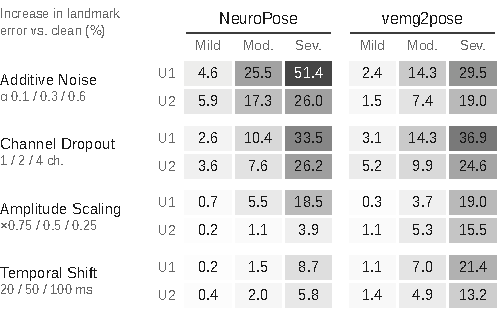
\includegraphics[width=\columnwidth]{fig2_heatmap.pdf}
  \caption{Increase in landmark error (\%) relative to each user and model's clean baseline (darker = larger). Rows: perturbation, with its swept parameter, and held out user; columns: model and severity. Noise std is $\alpha\,\sigma_c$, where $\sigma_c$ is the standard deviation of channel $c$ within the 5 s window. Noise and dropout cells average 5 seeds.}
  \Description{Grayscale heatmap of the percent increase in landmark error. Rows are 4 perturbations (additive noise, channel dropout, amplitude scaling, temporal shift), each split by 2 users; columns are 2 models (NeuroPose, vemg2pose), each at 3 severity levels. Darker cells are larger increases; the largest is 51.4\% (NeuroPose, U1, additive noise, severe).}
  \label{fig:heatmap}
\end{figure}
